\usepackage{hyperref}% NOTE - this is only a template without real arguments
\begin{entry}{Reorganization and Journal Update}{August 20, 2021}
    \objective 
    
    % What do you want to do?
    I need to establish mise en place for development of the ME.
    \outline
    
    %What steps are required?
    \begin{itemize}
        \item Reorganize my directory, put old files in an Outdated folder.
        \item Restart this journal.
        \item Update github README.md.
        \item Create ModelController.py
    \end{itemize}
    
    \procedures
    
    Should all be self explanatory.

    \parameters
    
    The point is to get ready to work without fumbling over old files or struggling to get my journal in order. The
    directory reorganization is pretty straight forward. Restarting this journal starts with this entry, but also
    organizing my journal update plan (which should be: update the journal every time you push, not commit.) I've
    already created ModelController.py and added the class outline to it in class form; most of the daily work from here
    on out will be adding classes and methods one by one, along with testing.

    The README needs refactored, and some documentation should be made public. I need to decide what gets links and
    what, if anything, gets added to the repository directly.
    
    \observations
    
    What happened?
    
    \data
    
    All recorded data, or where it can be found.
    
    \results
    
    Did you achieve your objective?
    
\end{entry}


%\begin{entry}{CMake Error running EGOT-DCM Dockerfile}{Dec 02, 2020}
%    \objective
%
%    Determine the cause of the CMake error while running the dockerfile and modify file to get it to successfully build.
%
%    \outline
%
%    \begin{itemize}
%        \item Try running to see if it was just Lorry or a machine issue.
%        \item If it is a machine issue, modify configurations to ensure interoperability.
%        \item If I get the error track down its cause and modify dockerfile to fix.
%        \item Repeat until all builds are successful.
%    \end{itemize}
%
%    \procedures
%
%    \begin{itemize}
%        \item \mint{console}|git clone https://github.com/EGoT-DCS-SunSpec-Modbus|
%        \item \mint{console}|docker build -f Dockerfile.buster -t egot-dcs .|
%        \item \mint{console}|docker container run -i egot-dcs|
%    \end{itemize}
%
%    \observations
%
%    \begin{error}{Cmake Error: No CMAKE\_CXX\_COMPILER found}
%        \begin{figure}[H]
%            \centering
%            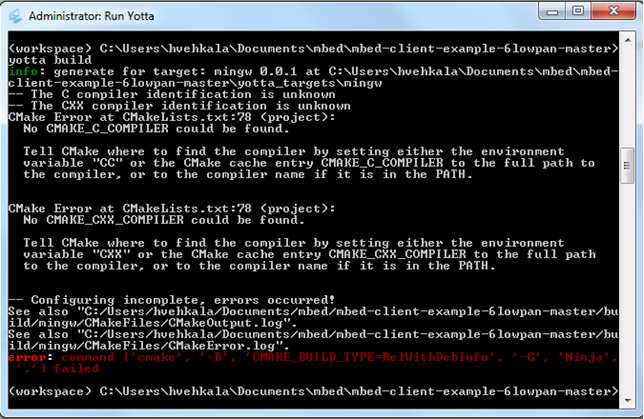
\includegraphics[height=4in]{Fall2020/Figures/cmake_error.png}
%        \end{figure}
%
%        Solution: what you need to do found at \cite{CMAKE-Forum}
%    \end{error}
%
%    \results
%
%    Short: No.
%
%    Long: Well...
%
%
%\end{entry}